\section{The Gisele process model analysis toolset\label{section:tool-clinical-pathway-analyzer}}

Safety-critical medical therapies call for well-defined processes. In particular, a clinical pathway is a documented process, based on medical protocols, guidelines and recommendations, centered on a specific patient class with similar needs. It generally involves multi-disciplinary teams and addresses clear clinical goals \cite{Middleton:2000}. 

The toolset presented in this section was motivated by the need for automated support to the building and analysis of models of clinical pathways and, more generally, mission-critical process models involving decisions. 

Guarded hMSCs were defined as a suitable process modeling language accessible to stakeholders; it has a formal semantics enabling a variety of model analysis \cite{Damas:2009, Damas:2011}. 

Those analyses are made at the g-LTS level; the toolset here thus relies on our synthesis algorithm for deriving g-LTS from g-hMSC, described in Section \ref{subsection:from-ghmsc-to-glts}.

A snapshot of the main screen of toolset front-end is shown in Fig.~\ref{image:gisele-tool}. A description of the toolset in action on a real medical case study can be found in \cite{Damas:2011}. This section discusses a few design decisions and highlights key points of the implementation. The main facilities provided by the toolset are the following:

\begin{figure}
\centering\scalebox{.525}{
  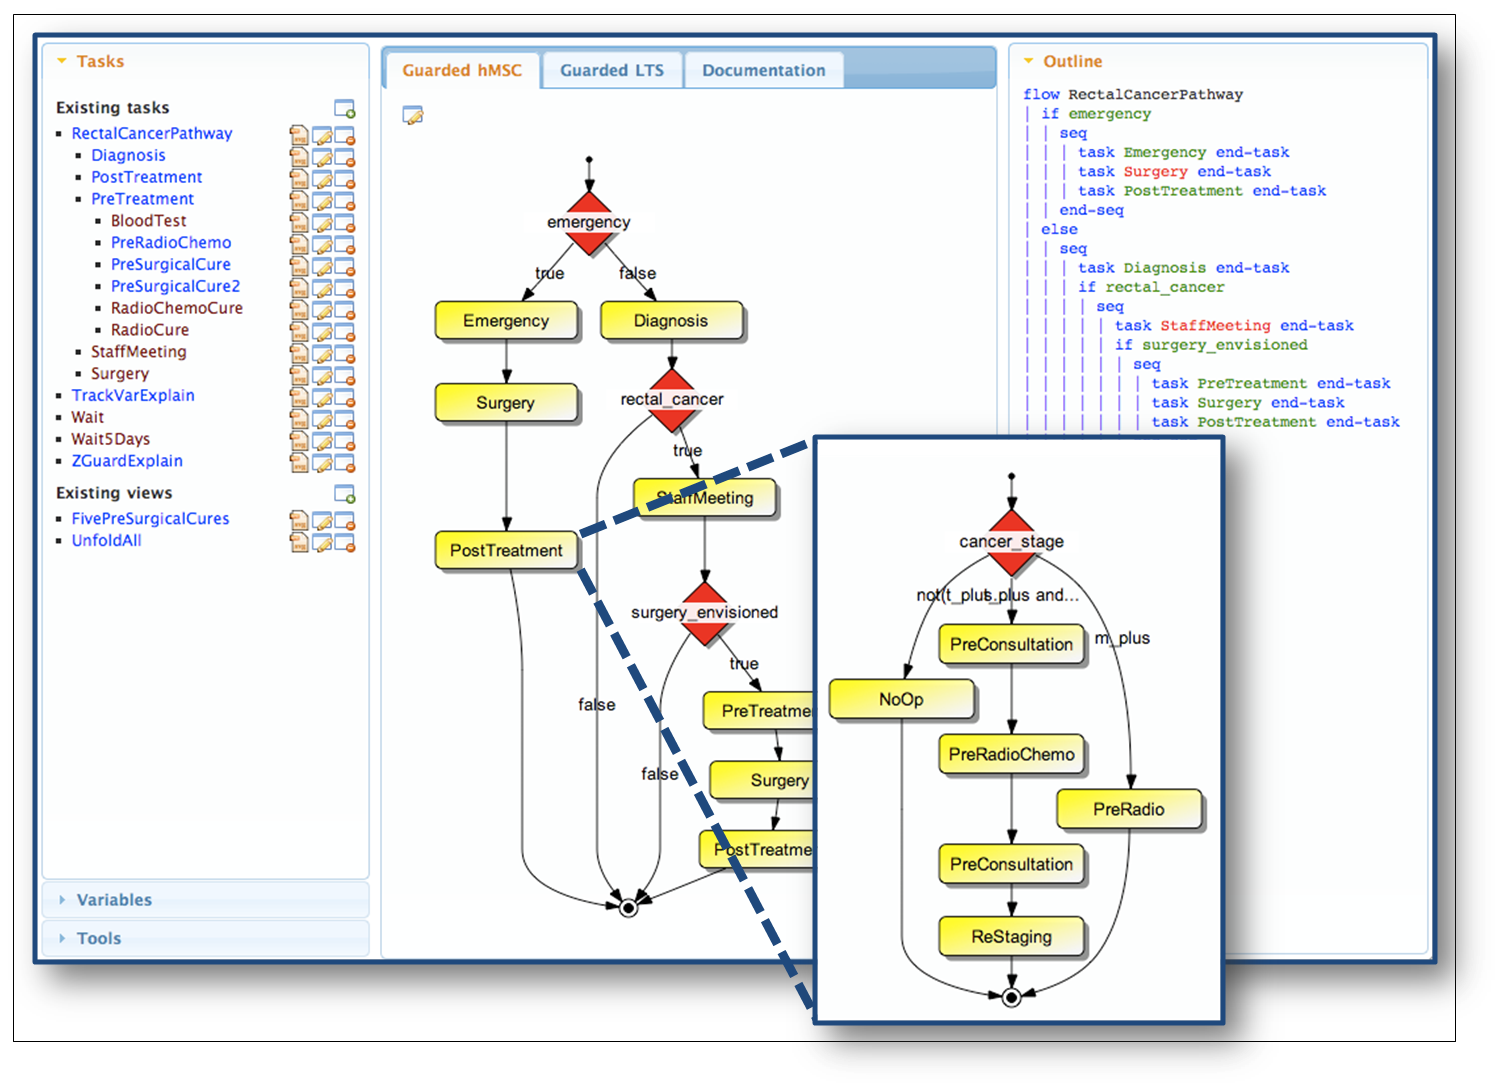
\includegraphics[trim=5mm 10mm 10mm 5mm, clip]{src/7-tool-support/images/gisele-tool}}
  \caption{The Gisele tool, a clinical pathway analyzer\label{image:gisele-tool}}
\end{figure}

\begin{itemize}
\item Editing and visualization of process models made of tasks and decision nodes defined on fluents and tracking variables (see Section \ref{section:background-process-models} and \cite{Damas:2009, Damas:2011}). Tasks can be successively refined in sub-processes, as illustrated in Fig.~\ref{image:gisele-tool}.
\item A variety of analyses, including (see \cite{Damas:2011} for details),
\begin{itemize}
\item Checking the completeness, non overlapping and satisfiability of guards at decision nodes.
\item Checking the adequacy of decision nodes, that is, whether these are made on fresh, accurate variable values.
\item Verifying pre-conditions of tasks.
\item Verifying non-functional process requirements such as time constraints, dose constraints, cost constraints, etc.
\end{itemize}
\item Visual means for eliciting process models; documenting them with stakeholders; unfolding process models for specific analyses; projecting them on specific patient classes, and so on.
\end{itemize}

\subsection*{Decision decisions}

The toolset has been designed for (1) eliciting critical processes during stakeholder interviews (2) analyzing them in real-time and (3) providing browsable process documentation. This implied two main design decisions:

\begin{description}
\item[Textual input] For allowing a rapid capture of process models by an analyst, a simple textual language is used as input language instead of a graphical language. This language essentially amounts to a guarded command language with constructs for iteration, loops, deterministic and non-deteministic choices, etc.

For example, the meeting scheduling process can be translated to this textual language as shown in Fig.~\ref{image:meeting-scheduling-gis}.

\begin{figure}[H]
\centering\scalebox{0.75}{
  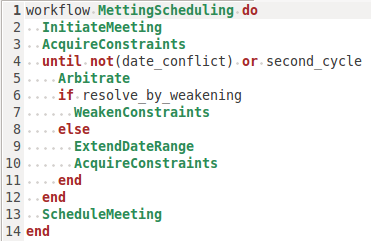
\includegraphics[trim=0mm 0mm 0mm 0mm, clip]{src/7-tool-support/images/meeting-scheduling-gis}}
  \caption{Meeting scheduling process encoded in the Gisele tool\label{image:meeting-scheduling-gis}}
\end{figure}

\item[Real-time proactive mode] Unlike the ISIS tool introduced in Section~\ref{section:tool-support-isis}, a proactive mode is used instead of reactive one with respect to checks and feedback:
\begin{itemize}
\item Reactive mode: in the ISIS tool, synthesis and checks are made ``on demand'': for example, the user explicitly launches consistency checks and receives dedicated feedback as a result (see Section \ref{section:tool-support-isis}).
\item Proactive mode: in the Gisele tool, the end-user navigates through the model thanks to the GUI that runs inside a web browser. Every time she looks at a task, the tree on the right panel provides real-time feedback about checks and their results, ``green'' means success, ``red'' means fail. The idea is inspired from continuous compilation chains in integrated development environments (IDE) such as Eclipse \cite{Gamma:2003}. Our experience suggests that this provides a natural and effective guidance in terms of continuous improvement of a process model. 

\end{itemize} 
\end{description}

\subsection*{Architecture}

The architecture of the toolset is shown in Fig.~\ref{image:gisele-tool-architecture}. The main modules are briefly described below:

\begin{figure}
\centering\scalebox{.5}{
  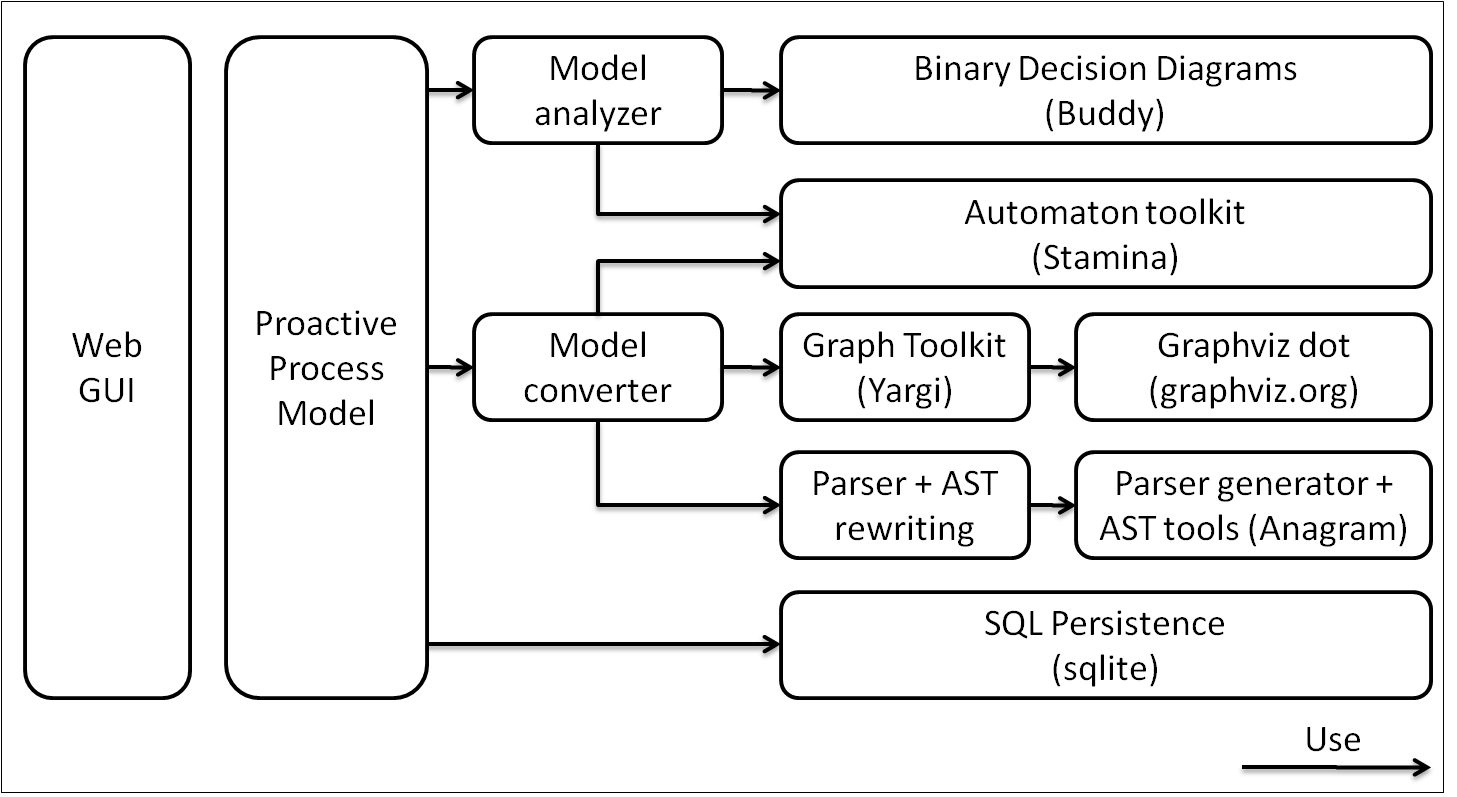
\includegraphics[trim=3mm 3mm 3mm 3mm, clip]{src/7-tool-support/images/gisele-tool-architecture}}
  \caption{Architecture of the Gisele tool\label{image:gisele-tool-architecture}}
\end{figure}

\begin{description}
\item[Web GUI] This module is the graphical user interface (GUI), that runs mostly inside a web browser. It is implemented in HTML5, CSS3 and Javascript \cite{Pilgrim:2011} and uses Scalable Vector Graphics for displaying guarded hMSCs \cite{Eisenberg:2002}. Thanks to the web services offered by the ``proactive process model'' module, the implementation of the GUI amounts to a simple model navigator, implemented internally with an MVC-like design pattern. 

The main screen of this navigator is made of three panels (see Fig~\ref{image:gisele-tool}). 
\begin{itemize}
\item The left panel gives a global outline of the process model and allows navigating it through. Links are provided to open and update task and fluent definitions.
\item The current task is displayed as a process graph in the middle panel; it is implemented in SVG. The layout of the graph is automatically computed server-side with the well-known \emph{dot} utility\footnote{available at http://graphviz.org}. Graph nodes can be clicked to navigate through task refinements.
\item The current task is also outlined through an annotated syntax tree in the right panel. Annotations provide analysis real-time feedback to the user; tasks and decision nodes for which at least one check fails are displayed in red. Clicking on a node in this tree gives a detailed analysis explanation and counterexamples showing why check fails.
\end{itemize}

\item[Proactive process model] Process models are made of several tasks in successive refinements, textual definitions such as the one in Fig.~\ref{image:meeting-scheduling-gis} for each of them, fluent definitions, task documentation, etc. This module implements the structure of such models which are kept persistent through the use of the SQLite database engine; the latter also provides support for model queries through SQL \cite{Date:1997}.

In addition, this module implements the proactive mode described in the design decisions through a design pattern inspired from logical data independence \cite{Date:2003}. Roughly, this pattern consists in hiding the difference between ``base'' information and ``computed'' one.

For example, the precondition is a base attribute of a task whose value is chosen by the analyst; the fact that this precondition is met or violated is another Boolean attribute whose value is computed as the result of a dedicated precondition check \cite{Damas:2011}. 

Systematically hiding this distinction between base and computed information helps implementing the proactive mode. Indeed, user feedback can be implemented through model queries. For example, ``what are all tasks whose precondition is violated?''. The module automatically triggers the model checks if needed to answer such query. To achieve this, it relies on other modules, which are described below.

\item[Model analyzer] This module implements the analyses detailed in \cite{Damas:2011}. They rely on various instantiations of an abstract fixpoint algorithm on g-LTS. Such analyses makes an intensive use of automata and binary decision diagrams with the help of dedicated libraries. The automaton toolkit is the one implemented for the Stamina contest (see Chapter \ref{chapter:stamina}). The \emph{Buddy} library is available at \verb|http://buddy.sourceforge.net|; being implemented in C, we use a interface binding for ruby available at \verb|http://people.cs.aau.dk/~adavid/BDD/|\footnote{both have been last retrieved on September 13 2011}.

For every process and sub-process instance, the proactive module automatically triggers the execution of an analysis as soon as its results are needed for answering a model query. Those results are kept as decorations on g-LTS states. The decorated states are kept as a cache for analysis results. This cache is cleaned up when a process definition is changed, by simply throwing its g-LTS away.

\item[Model converter] The implementation of the proactive module relies on specific algorithms for rewriting processes under multiple forms. For example, the textual definition of a task is parsed and kept as an abstract syntax tree (AST); rewritten as a guarded hMSC; converted to a graph for being displayed; compiled into an equivalent guarded LTS for analyses; and so on. 

This module implements conversion algorithms, relying on external libraries for parsing, manipulating ASTs, graphs and automata. This module also provides traceability support between the multiple views of the same process instance.
\end{description}
